  Nous avons mis en place un script bash qui permet de faire automatiquement une acquisition de photo et un traitement par notre algorithme de reconnaissance d'image. 

  Pour cela, il est nécessaire d'installer les logiciels cités ci-dessous et de brancher le boîtier NXJ et la caméra. 

  Le programme se lance grâce à l'exécutable COMPILEALL disponible à la racine de l'arborescence. 

  Ce programme effectue les étapes suivantes : 
  \begin{enumerate}
    \item Compilation des codes permettant de se connecter au boîtier NXJ, d'effectuer un mouvement avec le robot et de résoudre le cube. Dans notre cas, nous n'avons pas lancé directement la résolution du cube mais fait un affichage du résultat de l'initialisation comme montré dans la figure~\ref{fig:aff}.

    \item Capture des images du cube successive et déplacement du cube par le robot, 
    \item Utilisation de la reconnaissance d'image pour initialiser un cube. 
Le résultat de cette initialisation est sauvé dans un fichier, 
    \item Lecture de ce fichier par une classe Java intégrable dans la problématique générale du projet \rubic, 
    \item Affichage du résultat par la classe Java Main utilisé pour tester l'algorithme. 
  \end{enumerate}
    
  \begin{figure}[h!]
    \centering
    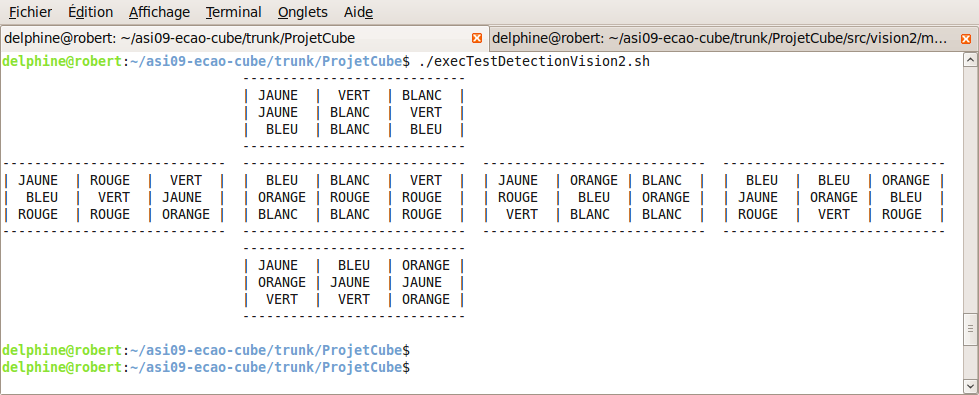
\includegraphics[width=0.8\linewidth]{./Images/affichage.png}
    \caption{Résultat de l'initialisation}
    \label{fig:aff}
   \end{figure}
  
  \textit{Remarque} Le résultat dans la figure~\ref{fig:aff} est obtenu à partir de la configuration 5 en Annexe~\ref{sec:Aconf}. 

  Le fichier permet la gestion des erreurs de détection de reflet et de détection de contour. 
  Ces erreurs sont traitées dans le programme Java qui récupère le résultat et provoque l'affichage de warning. 

  Nous n'avons pas ajouter la résolution du cube existante car nos résultats n'étaient pas satisfaisant, comme expliqué dans le chapitre~\ref{sec:avancement}. 

  \subsection*{Logiciels utilisés}

  Les logiciels à installer pour utiliser la reconnaissance d'image, en plus de ceux qui s'installent automatiquement grâce à instal.sh, sont : 
\begin{itemize}
  \item octave et octave-image pour l'algorithme de reconnaissance ; 
  \item gst pour la prise de photo ; 
  \item beep pour le signal sonore qui indique la fin de l'initialisation du cube est indique à l'utilisateur qu'il doit rallumer le boîtier NXJ pour la suite de la résolution du cube. En effet le temps de la reconnaissance d'image est suffisamment long pour que le boîtier NXJ s'éteigne, il faut alors le rallumer manuellement ; 
\end{itemize}

\textit{Remarque : } Si la caméra ne fonctionne pas, il est conseillé de baisser la résolution. 
